% $Date$
\documentclass[12pt,a4paper]{article}
\usepackage[polish]{babel}                      % Język polski
\usepackage[utf8]{inputenc}                     % Kodowanie dokumentu
\usepackage[T1]{fontenc}                        % Kodowanie fontów
%\usepackage{lmodern}
\usepackage{times}                              % Font wektorowy
\usepackage[cm]{fullpage}                       % Cała szerokość strony
\usepackage[pdftex,bookmarks,colorlinks]{hyperref} % Linki w dokumencie PDF
\usepackage{indentfirst}                        % Wcięcia akapitów
\usepackage{graphicx}                           % Grafika w png, jpeg, gif
%\pagestyle{headings}
%\graphicspath{{png}}                            % Szuka grafik w katalogu png
\frenchspacing                                  % Odstępy międzyzdaniowe

\title{ConvML 1.2}
\author{Marcin Kacprzak \and Piotr Kulinowski}
\date{\today}

\begin{document}

\maketitle
\tableofcontents

\section{Wstęp}
Ten dokument zawiera opis funkcji i składni języka ConvML.  ConvML jest językiem
do zapisu strukturalnego modelu przenośnika taśmowego w XML'u[XML10].

Potrzeba opracowania modelu strukturalnego przenośnika taśmowego wynikła z
informatycznej konieczności wprowadzenia procedury zapisu pełnej informacji o
urządzeniu, która jednoznacznie i spójnie opisywałaby parametry
techniczno-ruchowe i konfigurację przenośnika taśmowego.  Ze względu na
uniwersalność zapisu i chęć popularyzacji modelu strukturalnego wprowadzono
anglojęzyczne nazewnictwo poszczególnych podzespołów.

\begin{figure}
  \centering
  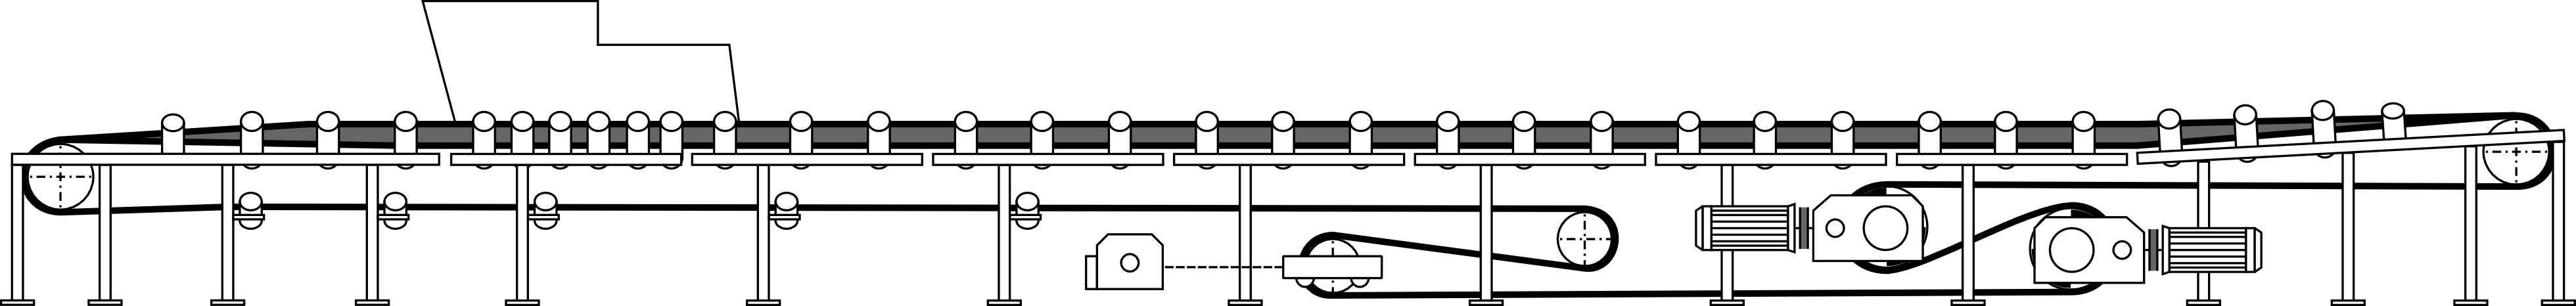
\includegraphics[width=\textwidth]{png/przenosnik}
  \caption{Podstawowe podzespoły przenośnika taśmowego}
  \label{fig:przenosnik}
\end{figure}

Do opracowania systemu zapisu modelu strukturalnego przenośnika taśmowego
wykorzystano język XML Schema [?89], ułatwiający definiowanie struktury i
kolejności podzespołów przenośnika taśmowego (Tabela 4 1) oraz umożliwiający w
łatwy sposób jego adaptację na platformie informatycznej.  Istotną cechą modelu
strukturalnego jest praktycznie nieograniczona możliwość jego rozbudowy, bez
utraty przejrzystości struktury.  Każdy z elementów posiada grupę atrybutów
opisujących jego cechy, mogące być zarówno parametrami technicznymi jak i
ekonomicznymi.

\section{Konwencje}
Nazwa ConvML pochodzi od Conveyor Meta Language.  Typowy dokument ConvML ma
postać pliku tekstowego o rozszerzeniu xml lub convml.  Zalecane kodowanie to
UTF-8.

Dokument ConvML do zapisu informacji o strykturze przenośnika wykorzystuje
elementy, a do zapisu właściwości używane są atrybuty języka XML.  Elementy w
języku ConvML mogą zawierać inne elementy oraz atrybuty, nie używa się natomiast
tekstu zawartego pomiędzy znacznikami do zapisu informacji o przenośniku
taśmowym.

Elementy języka ConvML należą do przestrzeni nazw:
http://www.entertech.com.pl/bcml.

\section{Struktura dokumentu: element ConvML}

Głównym elementem dokumentu jest element ConvML. Podelementy Meta oraz Types są
opcjonalne. Element BeltConveyor musi wystąpić co najmniej raz aby dokument był
poprawny. Przykładowa instancja dokumentu może mieć następującą postać:

\begin{verbatim}
<?xml version="1.0" encoding="utf-8"?>
<ConvML version="1.2">
  <Meta />
  <Types />
  <BeltConveyor />
</ConvML>
\end{verbatim}  

\subsection{ConvML}

\begin{figure}[h]
  \centering
  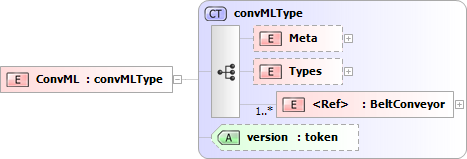
\includegraphics[width=0.6\textwidth]{png/convml_xsd2}
  \caption{Definicja elementu ConvML}
  \label{fig:convml-xsd}
\end{figure}

\paragraph{Definicje atrybutów:}
\begin{description}
\item[version] zastosowana w dokumencie wersja języka ConvML.
\end{description}

\end{document}
